\index{Component!Names!Delete}
\index{Delete!Component Names}

When you reassign component names in the \gdcompnamesview{}, you automatically create new component names if the name you enter did not previously exist in the \gdproject{}. 

Larger \gdprojects{} can often end up with a number of component names that are no longer used. You can see and delete these names in the \gdcompnamebrowser{}. 
The names in the \bxname{Unused Component Names} category  (\bxfigref{compnamebrowser}) are not used anywhere in this \gdproject{} -- they are not present in any \gdcases{} and they have not been mapped to any technical names from the \gdaut{} in the \gdomeditor{}.

\begin{figure}[h]
\begin{center}
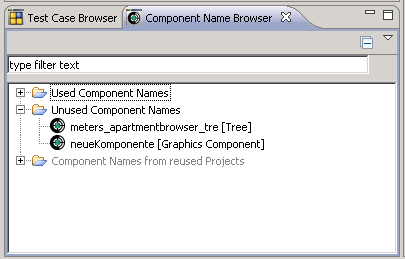
\includegraphics{Tasks/Compnames/PS/compnamebrowser}
\caption{The \gdcompnamebrowser{}}
\label{compnamebrowser}
\end{center}
\end{figure} 

To delete unused component names, select the name you want to delete and select:\\
\bxmenu{Delete}{}{}\\
from the context-menu. 

\bxtipp{To cleanup component names that are only used in mappings, or that are no longer used for a specific \gdaut{}, use the function \bxname{Cleanup unused component names} in the \gdomeditor{} {\bxpref{TasksOMCleanup}}.}
